\begin{titlepage}
\begin{center}

\includegraphics[height=2cm]{tue-logo-high}\\
%\LARGE
%Eindhoven University of Technology \\
\large
Department of Mathematics and Computer Science  \\
Applied Geometric Algorithms Research Group

\vspace*{10cm}

\setlength{\TPHorizModule}{1mm}
\setlength{\TPVertModule}{\TPHorizModule}
% Set the Paragraph Indent to zero, so the first line is not Indented
% Back-up the current value so it can be put back at the end of the title page
\newlength{\backupparindent}
\setlength{\backupparindent}{\parindent}
\setlength{\parindent}{0mm}
% Begins a textbox at 72 mm from the left of the edge of the paper and 89 mm from the top
% The width of the textbox is 95 mm (167 - 72 mm)
% The height of the box cannot be defined, so it is your task to keep the text not too long
\begin{textblock}{115}(52,89)
    \vspace*{1mm}
    \huge
    \textbf{\doctitle \\}
    \Large
    \vspace*{10mm}
    \me\\
    \vspace{30mm}

    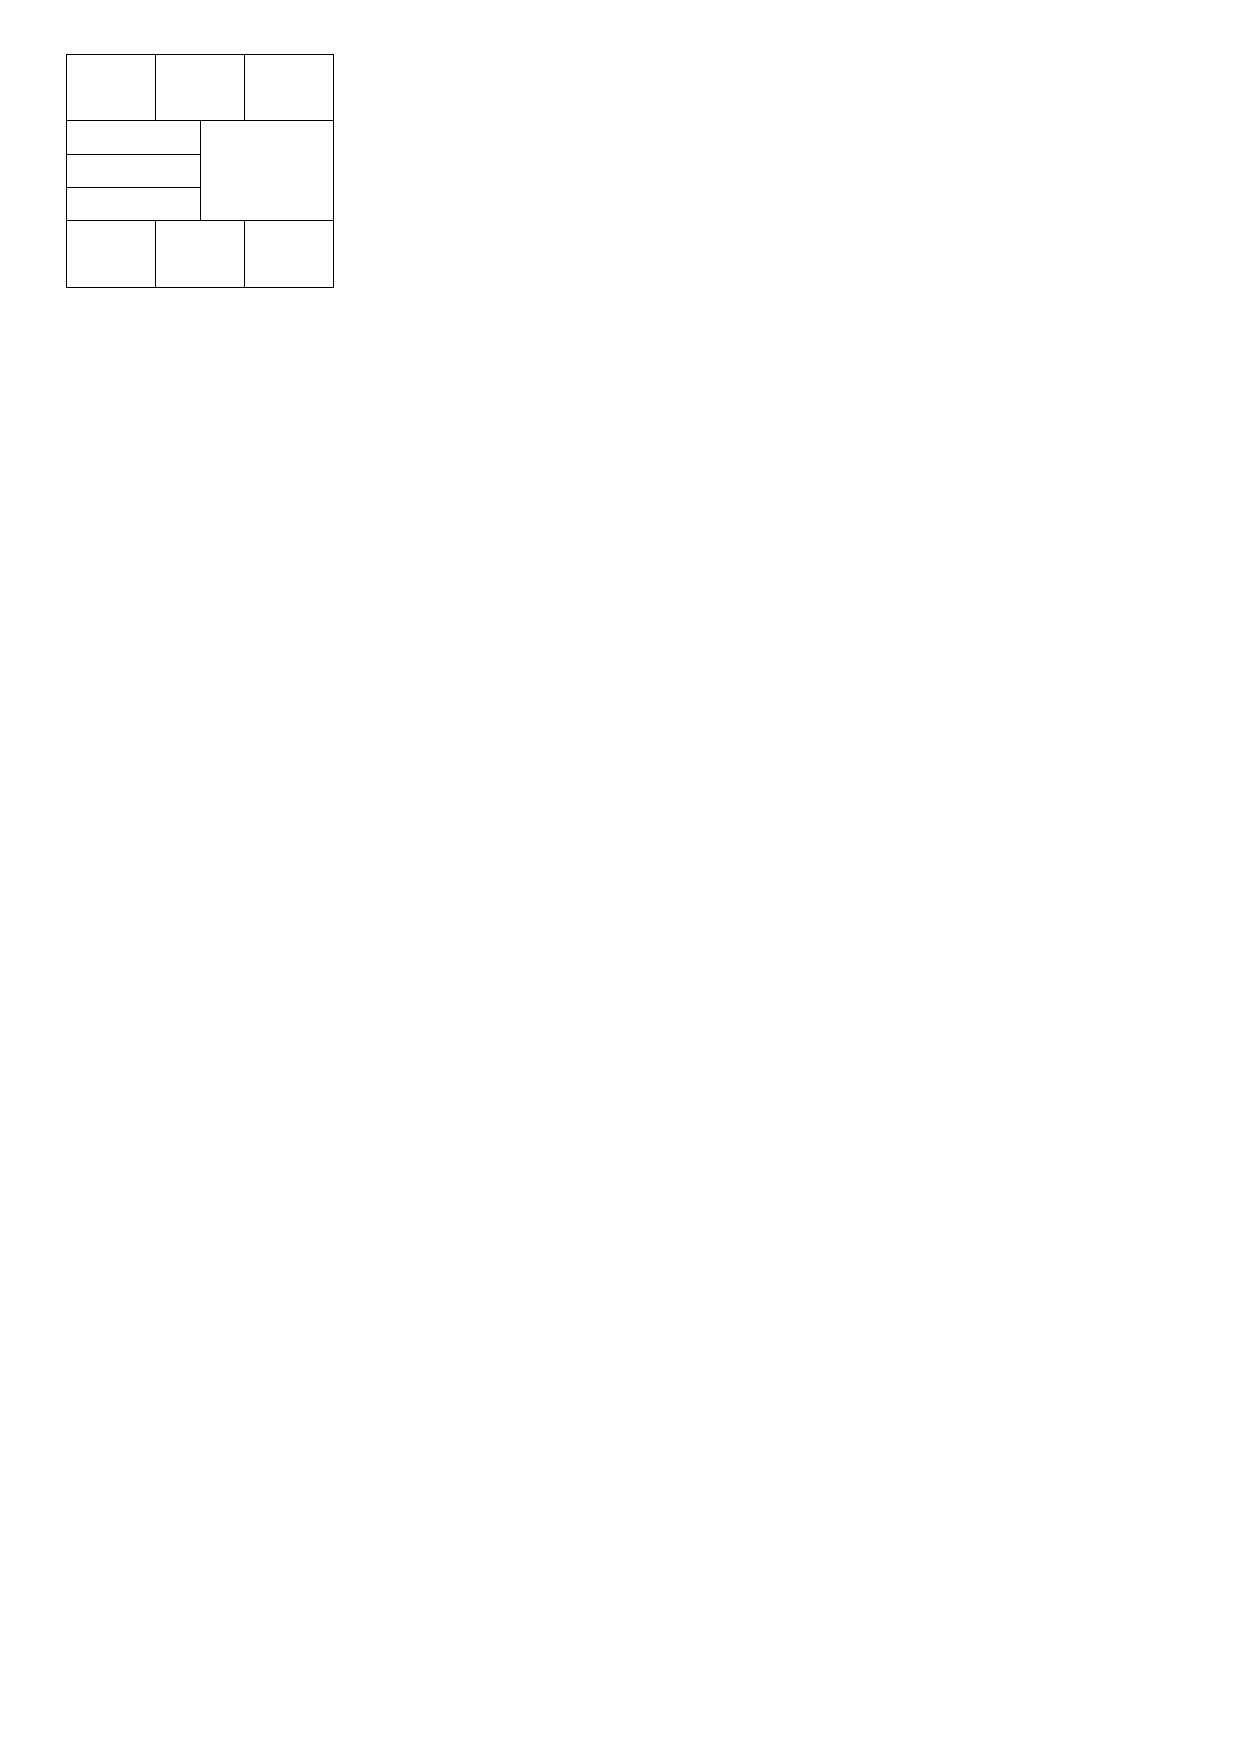
\includegraphics{titleimage.pdf}

\end{textblock}

\vspace{40mm}

\large
\hfill
\begin{minipage}{0.63 \textwidth}
Supervisors:\\
\begin{tabular}{ll}
    \firstCommitteeMember\\
    \secondCommitteeMember\\
    \thirdCommitteeMember\\
    \fourthCommitteeMember\\
\end{tabular}
\end{minipage}

\vfill
%\docdate \\
\large

Eindhoven, \ \monthYear\\

\href{mailto:sander@sanderbeekhuis.nl}{\texttt{sander\MVAt sanderbeekhuis.nl}}


% Put the Paragraph Indent back to its original value
\setlength{\parindent}{\backupparindent}
\end{center}
\end{titlepage}
